\documentclass[a4paper, 12pt]{article}
\usepackage{titling}
\usepackage{array}
\usepackage{booktabs}
\usepackage{enumitem}
\usepackage{graphicx}
\usepackage{hyperref}
\usepackage{amssymb}
\usepackage{listings}
\usepackage{color} %red, green, blue, yellow, cyan, magenta, black, white
\setlength{\heavyrulewidth}{1.5pt}
\setlength{\abovetopsep}{4pt}
\setlength{\parindent}{0pt}
\graphicspath{{.}}

\usepackage[margin=1in]{geometry}
\definecolor{mygreen}{RGB}{28,172,0} % color values Red, Green, Blue
\definecolor{mylilas}{RGB}{170,55,241}
% Must be after geometry
\usepackage{fancyhdr}
\pagestyle{fancy}
\fancyhf{}
\rhead{NN Homework 4}
\lhead{P.Lukin, I. Vishniakou, E. Ovchinnikova}
\cfoot{\thepage}

\setlength{\droptitle}{-5em}

\title{Neural Networks  \\
				- Homework 4 -}
\author{Petr Lukin, Ivan Vishniakou, Evgeniya Ovchinnikova}
\date{Lecture date: 24 October 2016}

\begin{document}

%-------------------------------------------------------------------------------
\lstset{language=Matlab,%
    %basicstyle=\color{red},
    breaklines=true,%
    morekeywords={matlab2tikz},
    keywordstyle=\color{blue},%
    morekeywords=[2]{1}, keywordstyle=[2]{\color{black}},
    identifierstyle=\color{black},%
    stringstyle=\color{mylilas},
    commentstyle=\color{mygreen},%
    showstringspaces=false,%without this there will be a symbol in the places where there is a space
    numbers=left,%
    numberstyle={\tiny \color{black}},% size of the numbers
    numbersep=9pt, % this defines how far the numbers are from the text
    emph=[1]{break},emphstyle=[1]\color{red}, %some words to emphasise
    %emph=[2]{word1,word2}, emphstyle=[2]{style},
}

%-------------------------------------------------------------------------------

\maketitle

\section{Mind map}

\begin{figure}[h]
  \centering
  \caption{Competitive neural network with feedforward connections.\label{fig:NNstatistical}}
  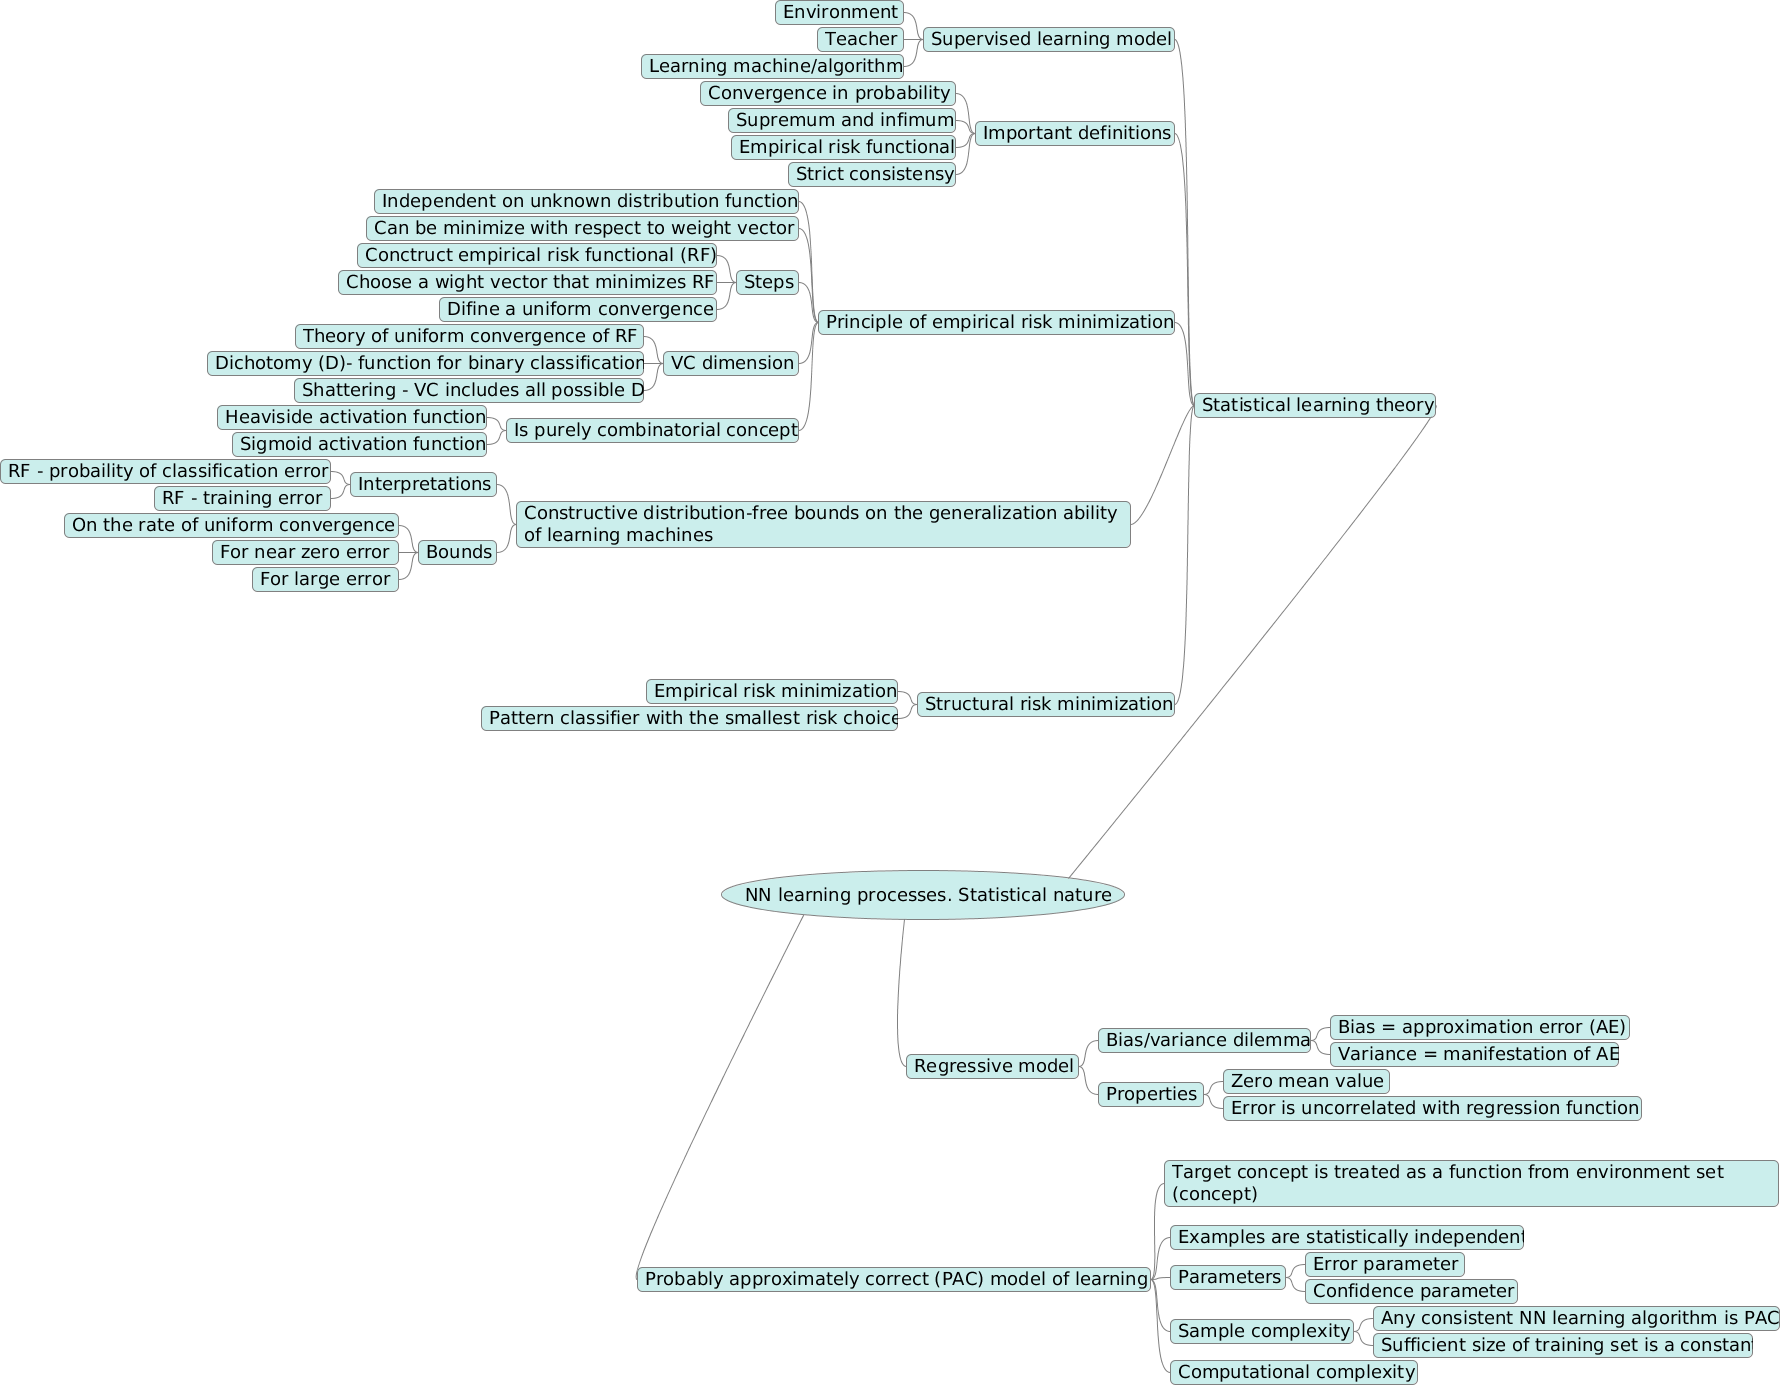
\includegraphics[width=1.0\textwidth]{NNstatistical}
\end{figure}

\section{Exercises}

\subsection{Exercise 2.1}




\end{document}
